\subsection{بخش ر}
در این بخش با محدود کردن زاویه پیش‌بین بین ۰/۰۵ رادیان، موشک از پهنای باند خارج نشد. نتایج در ادامه آمده است.

\begin{figure}[H]
	\centering
	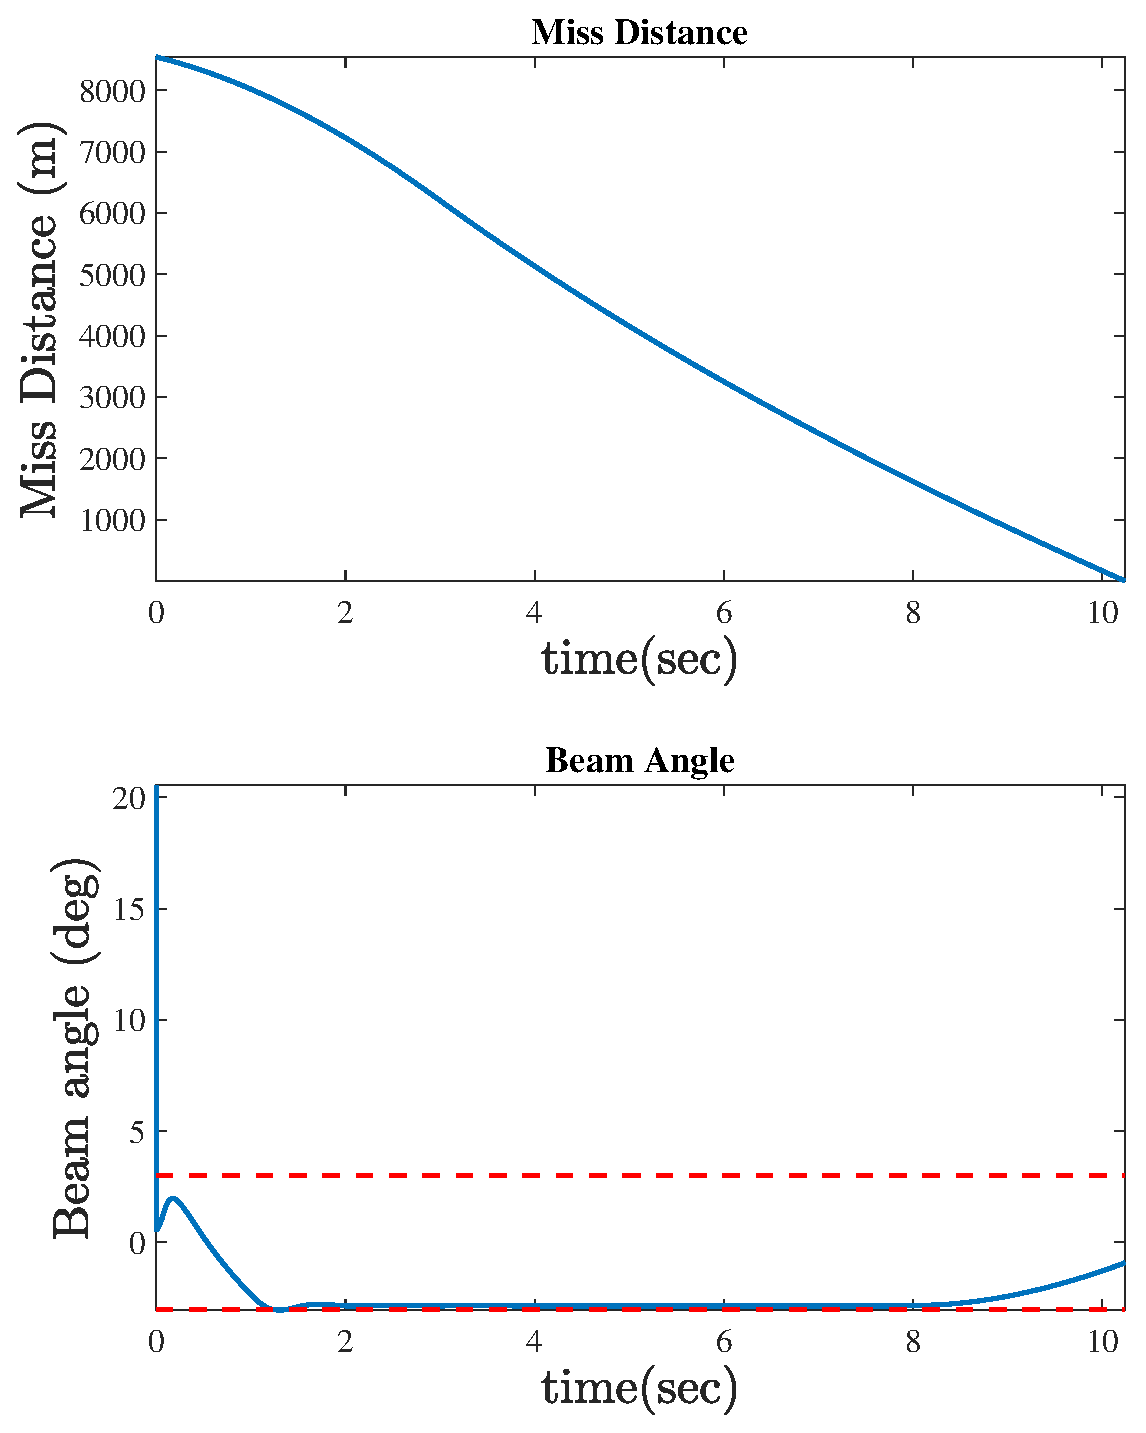
\includegraphics[width=.75\linewidth]{../Figure/l/miss_distance_with_time}
	\caption{تاریخچه فاصله ازدست‌دهی و پهنای بیم مورد نیاز در طی مسیر}
\end{figure}

\begin{figure}[H]
	\centering
	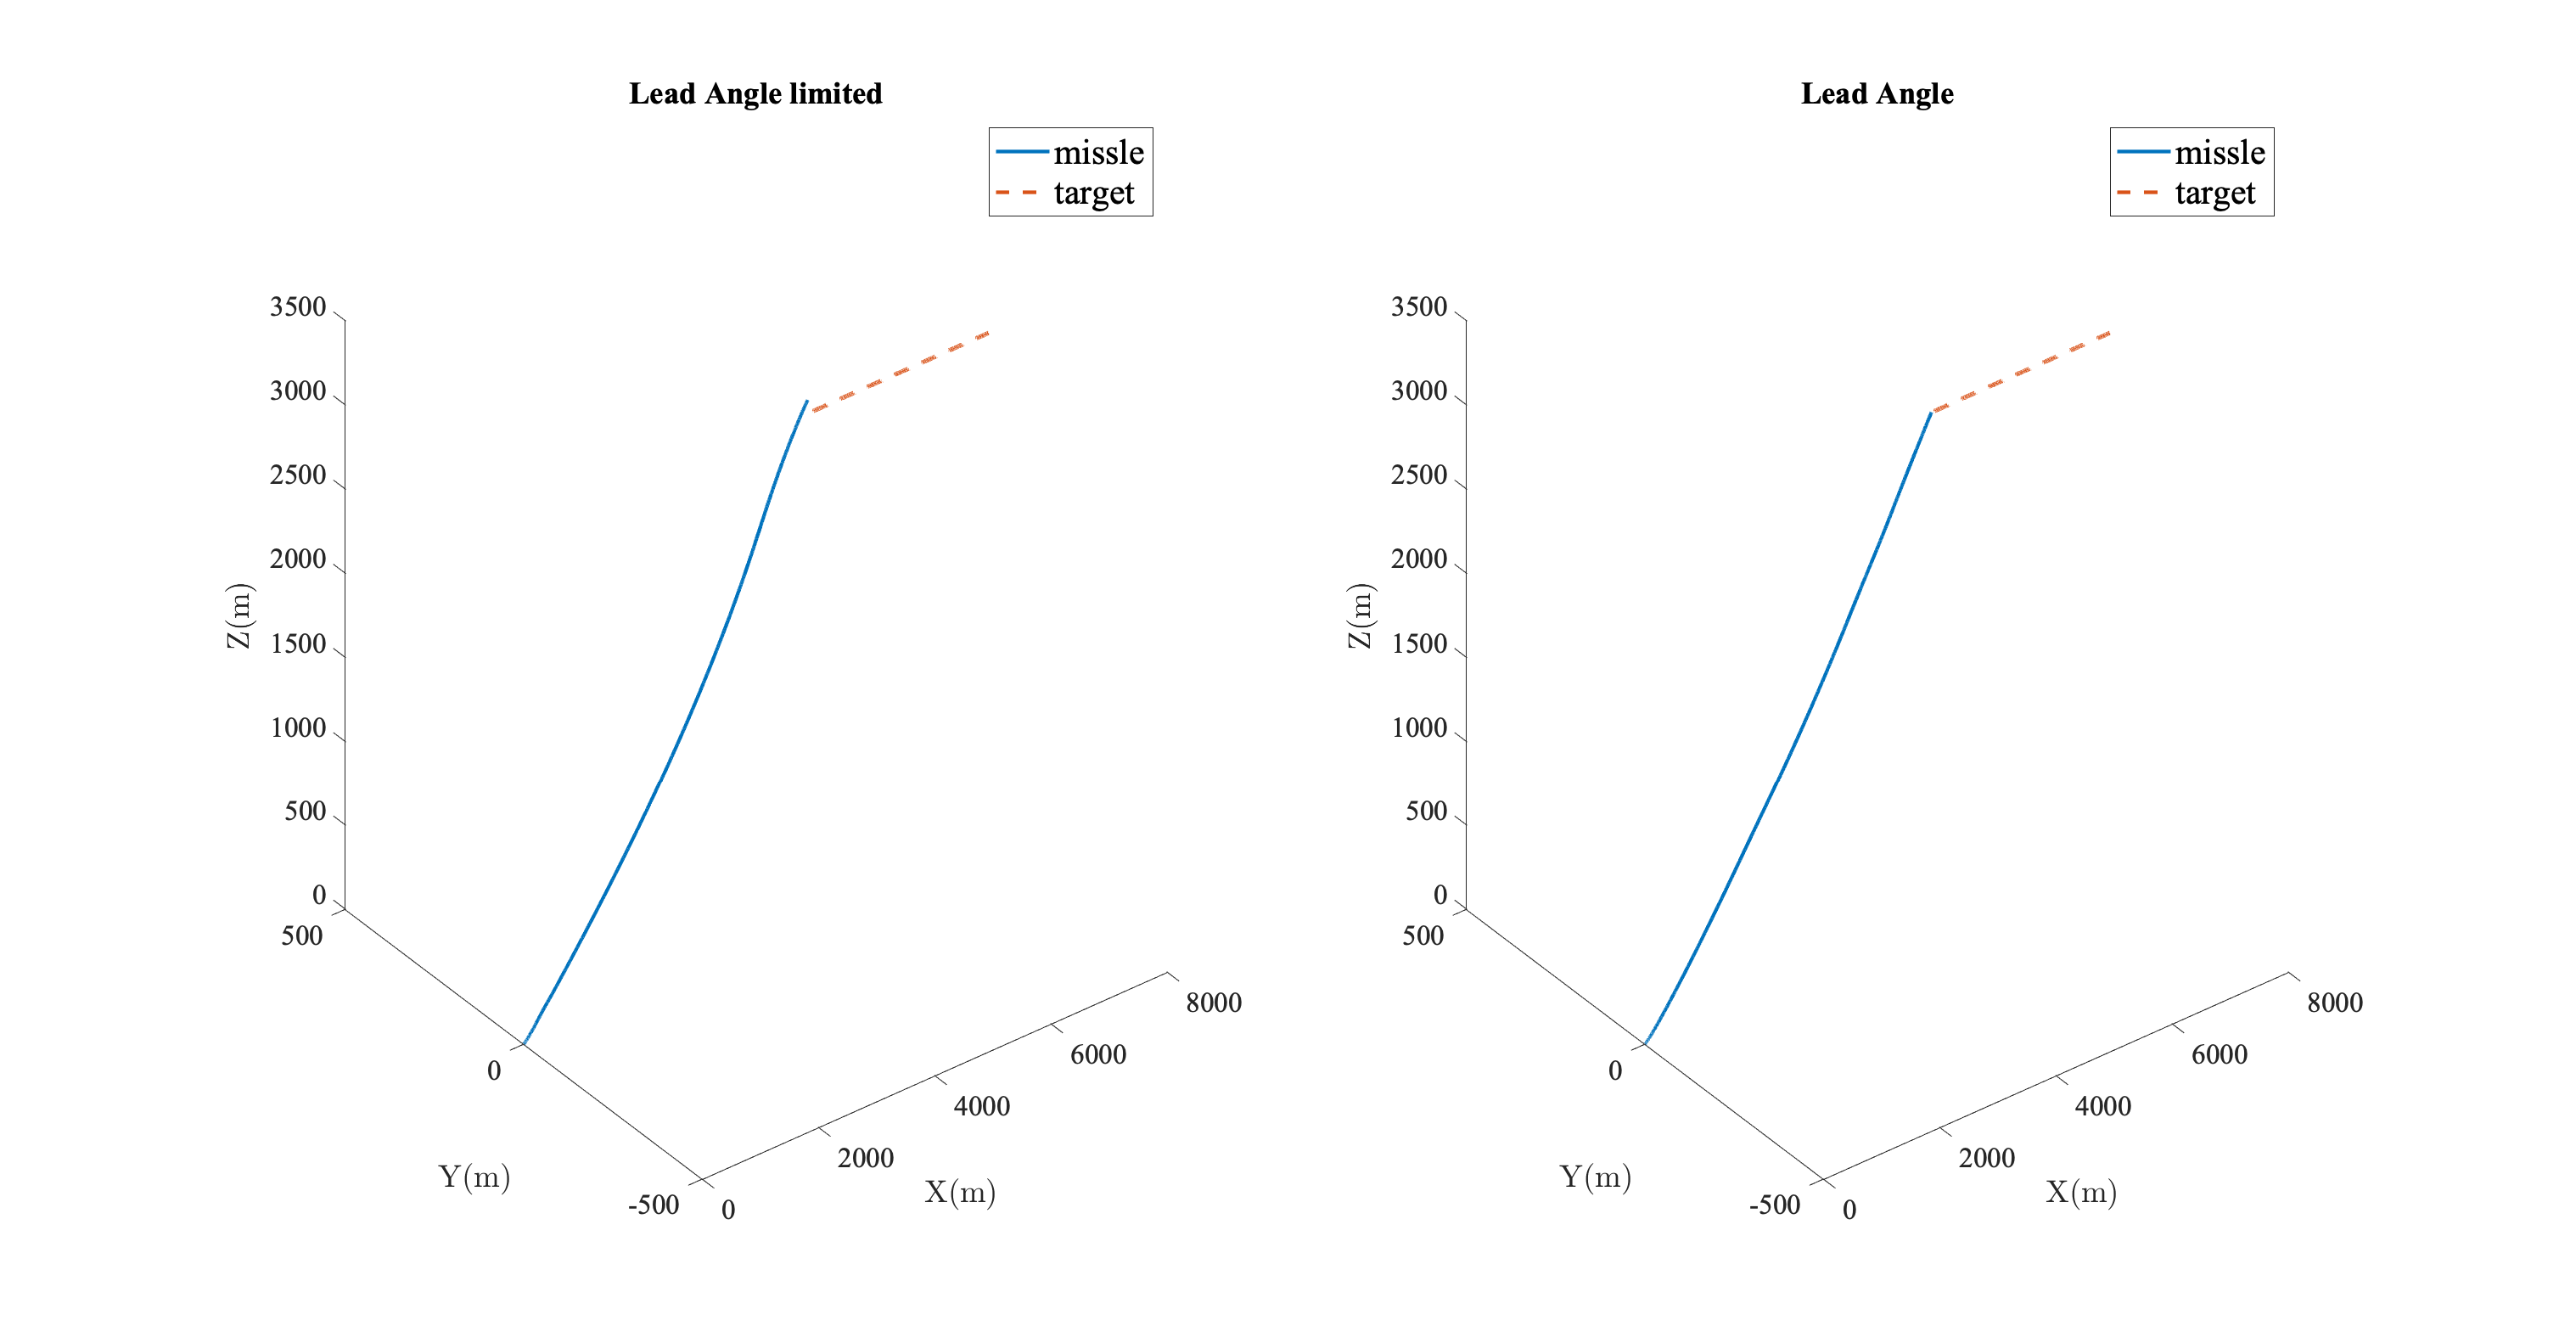
\includegraphics[width=\linewidth]{../Figure/l/3DoF_missle_vs_target_state_lead_angle_limited}
	\caption{مقایسه موقعیت موشک و هدف به صورت سه بعدی در دو نمودار  در قانون هدایت فرمان به خط دید همراه با محدود کننده زاویه پیش‌بین
	}
\end{figure}


\begin{figure}[H]
	\centering
	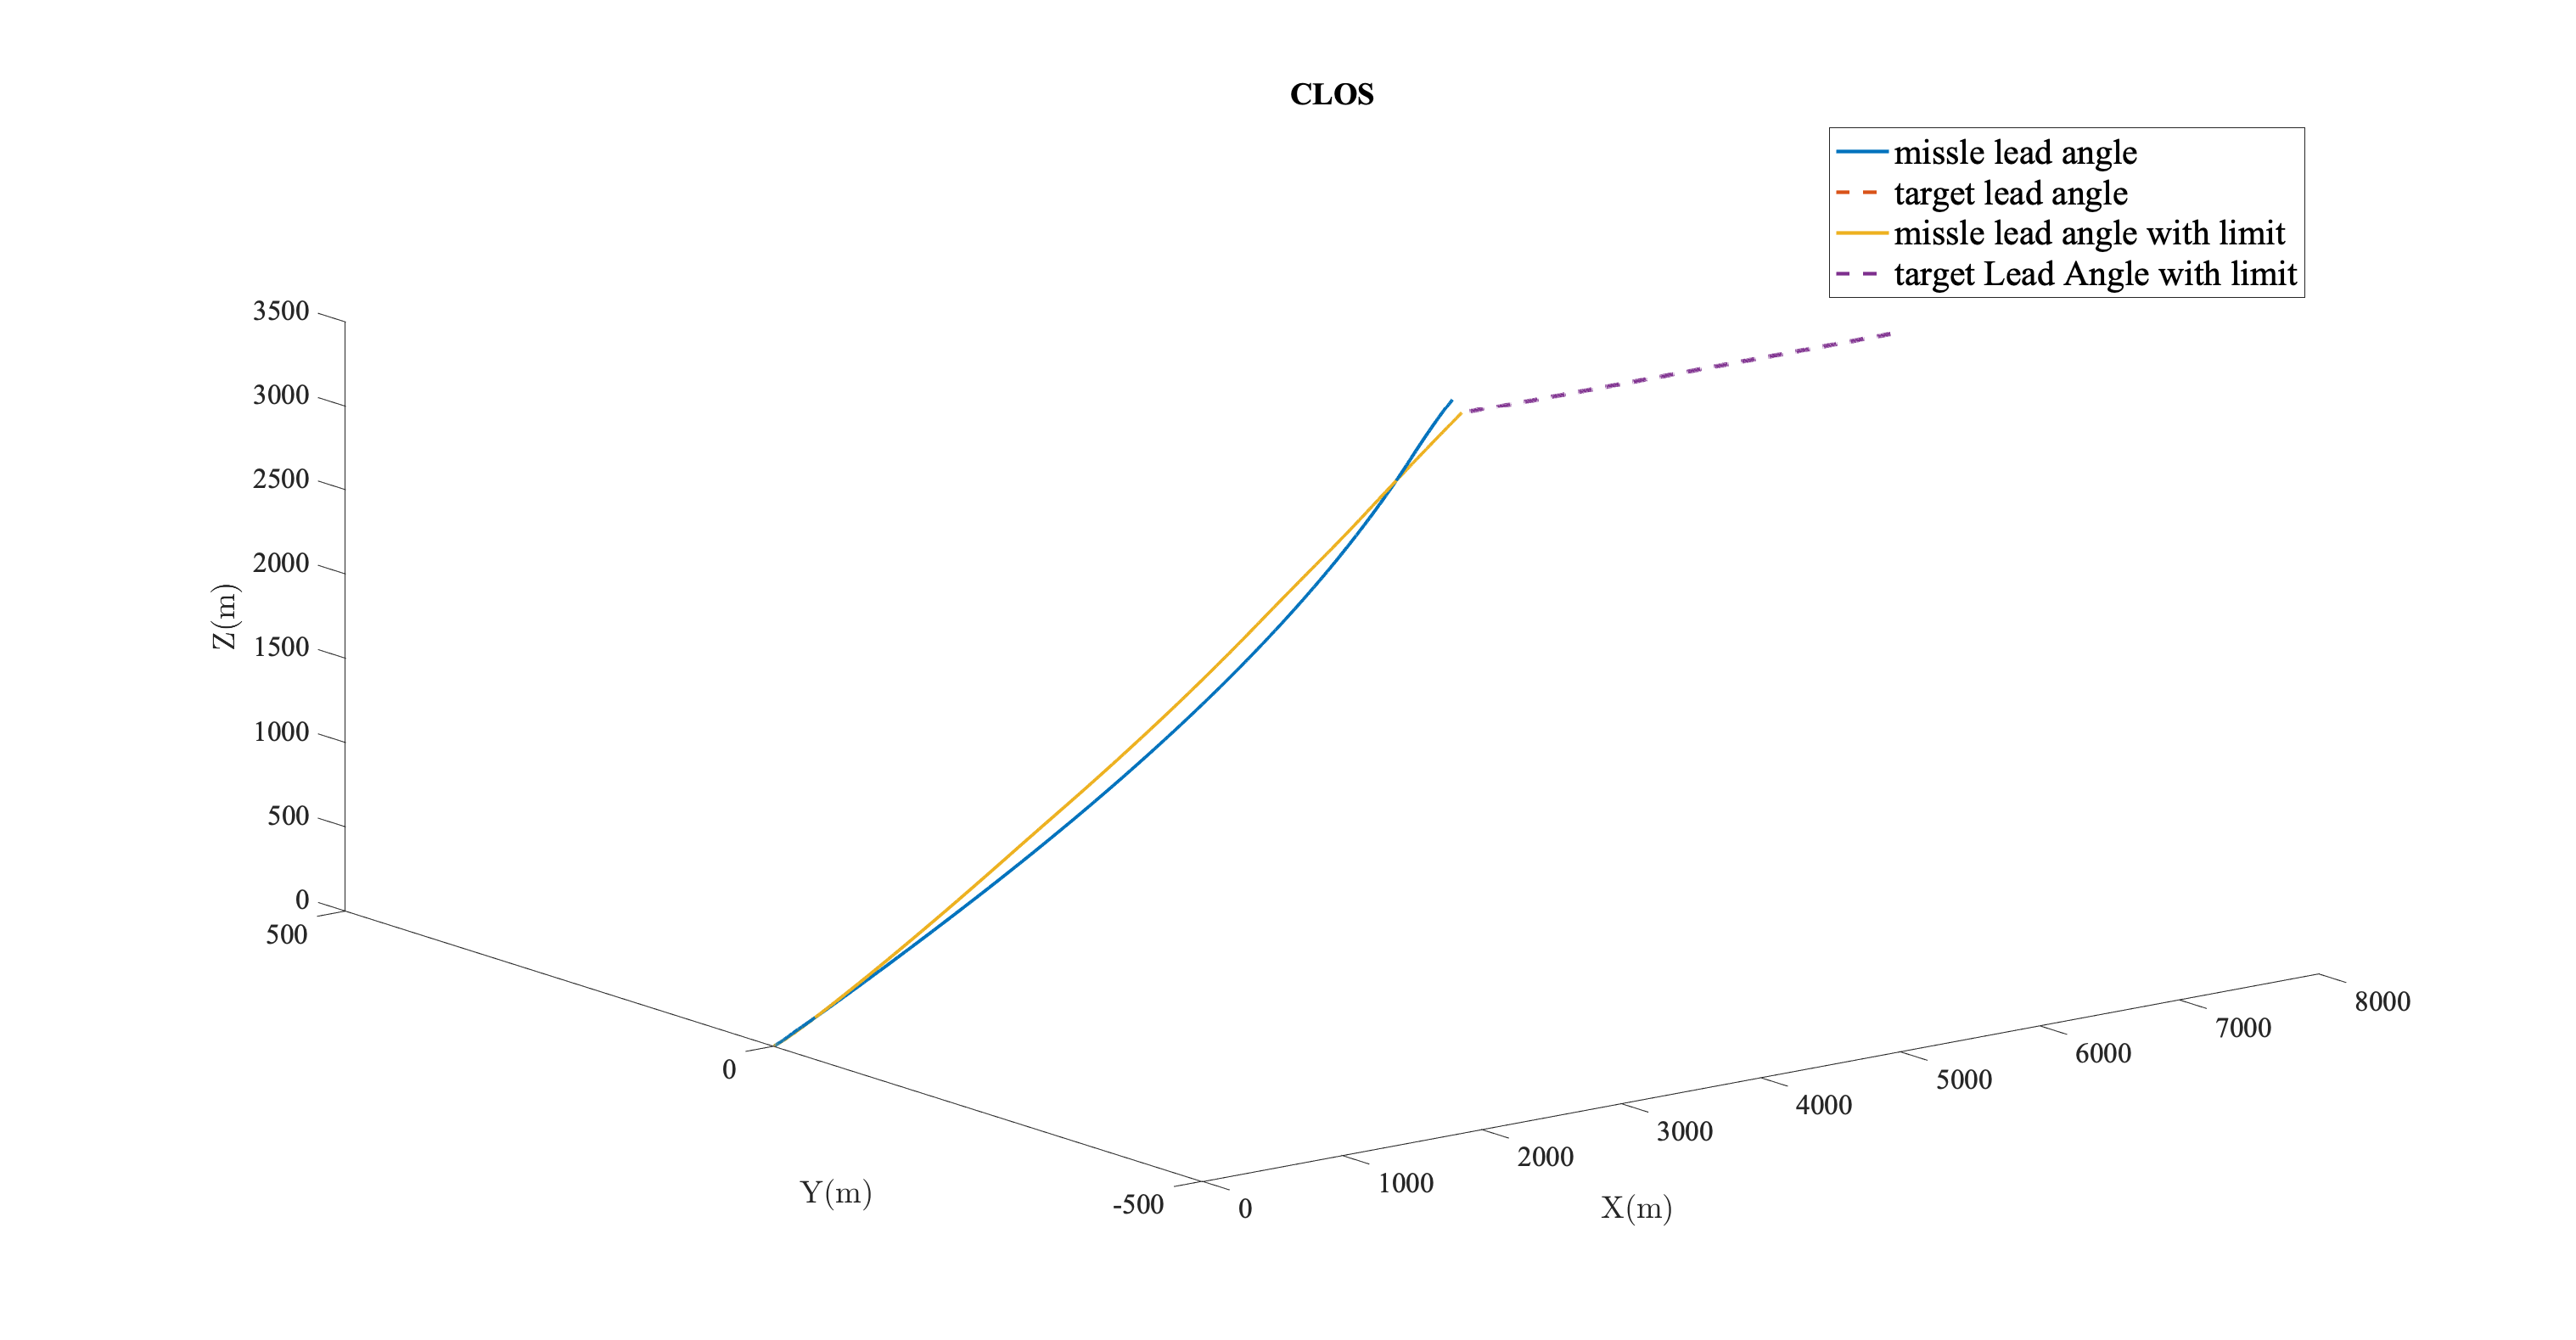
\includegraphics[width=\linewidth]{../Figure/l/3DoF_missle_vs_target_state_lead_angle_limited_all_in}
	\caption{مقایسه موقعیت موشک و هدف به صورت سه بعدی در یک نمودار در قانون هدایت فرمان به خط دید همراه با محدود کننده زاویه پیش‌بین
	}
\end{figure}

\begin{figure}[H]
	\centering
	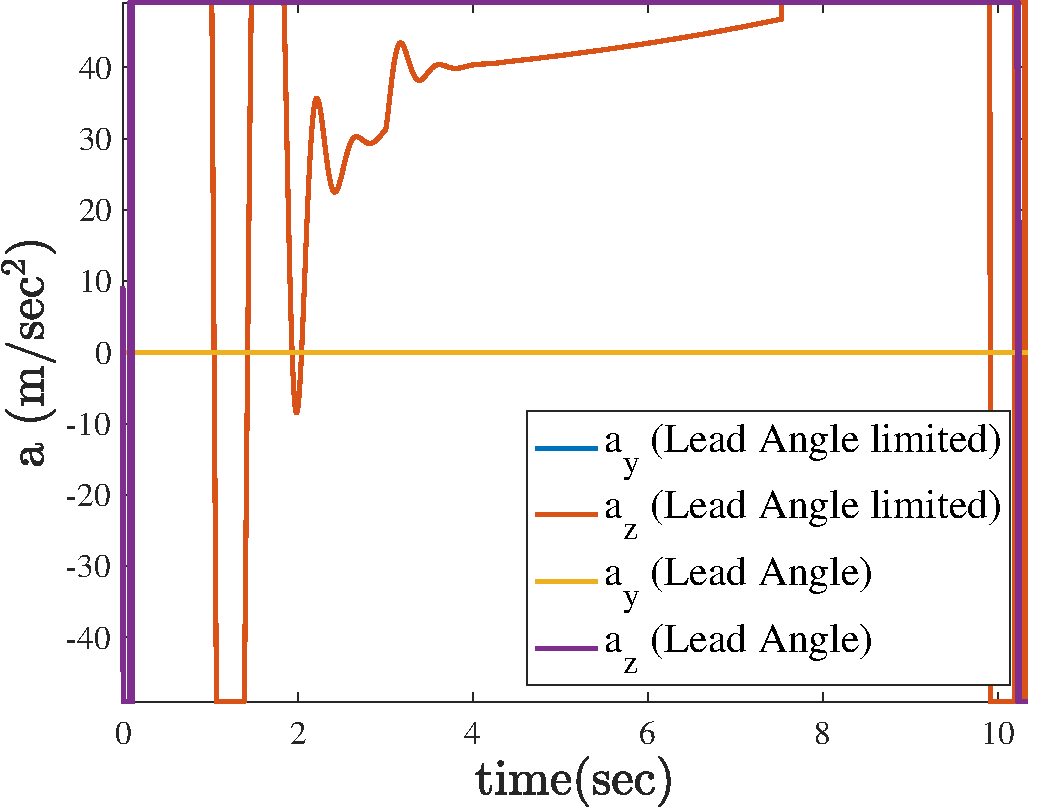
\includegraphics[width=.75\linewidth]{../Figure/l/command}
	\caption{مقایسه فرمان موشک در قانون هدایت فرمان به خط دید همراه با محدود کننده زاویه پیش‌بین}
	
\end{figure}

\begin{figure}[H]
	\centering
	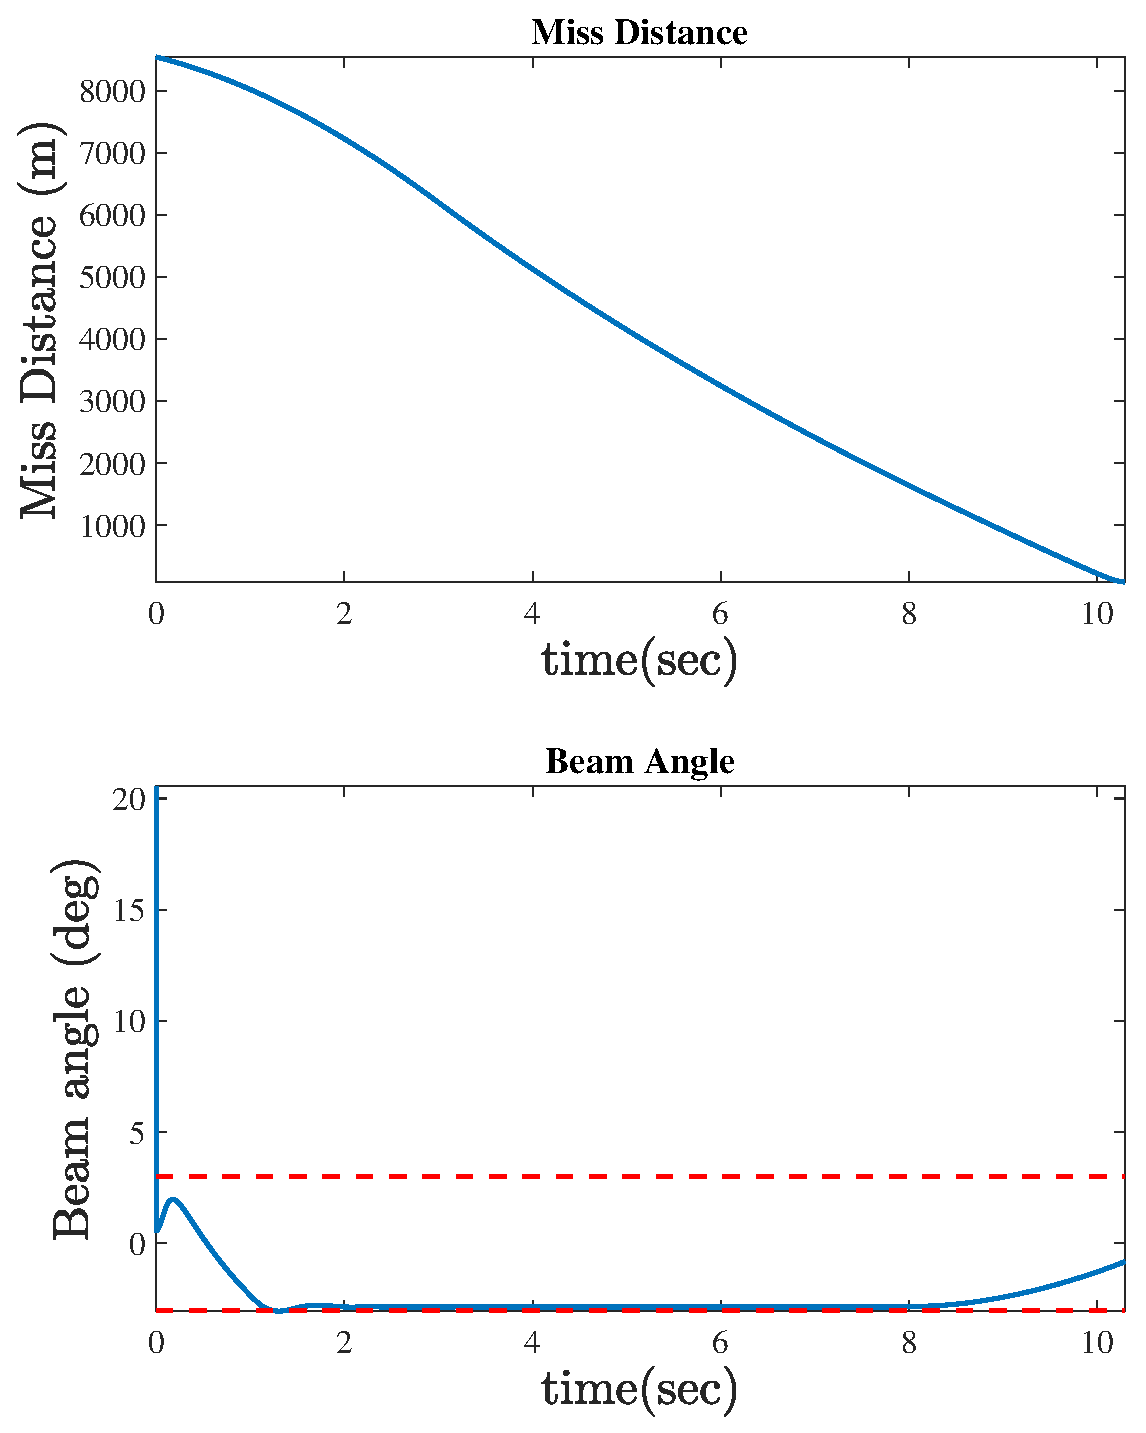
\includegraphics[width=.75\linewidth]{../Figure/l/miss_distance}
	\caption{مقایسه فاصله ازدست‌دهی موشک در قانون هدایت فرمان به خط دید همراه با محدود کننده زاویه پیش‌بین}
\end{figure}

